\captionsetup{justification=centering}
\begin{figure}[H]
    \begin{subfigure}{1\textwidth}
        \centering
        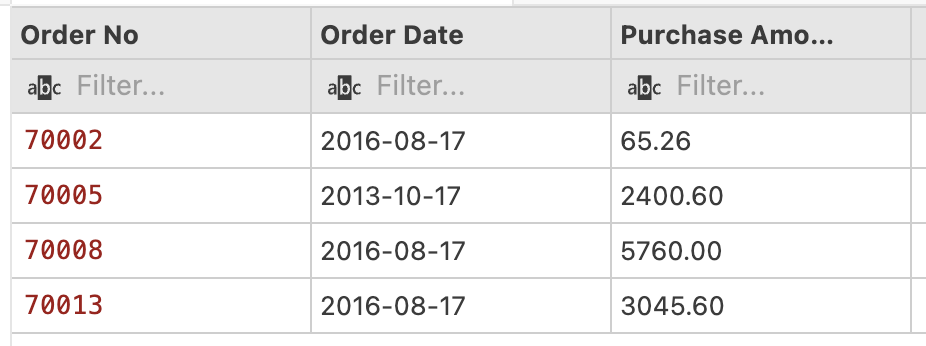
\includegraphics[width=.6\linewidth]{images/output/q1.png}
        \caption*{Order number, order date \& the purchase amount for
            order(s) which will be delivered by the salesman with ID 5001}
        \label{fig:q1}
    \end{subfigure}
    \begin{subfigure}{1\textwidth}
        \centering
        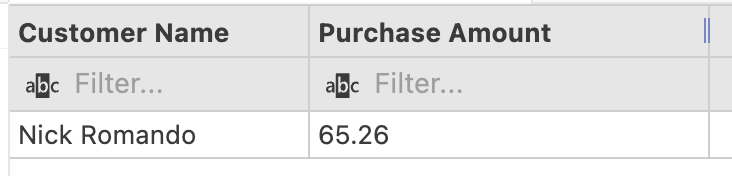
\includegraphics[width=.6\linewidth]{images/output/q2.png}
        \caption*{The customer name \& price of the cheapest items(s) using
            sub-query}
        \label{fig:q2}
    \end{subfigure}
    \vspace*{10mm}
    \begin{subfigure}{1\textwidth}
        \centering
        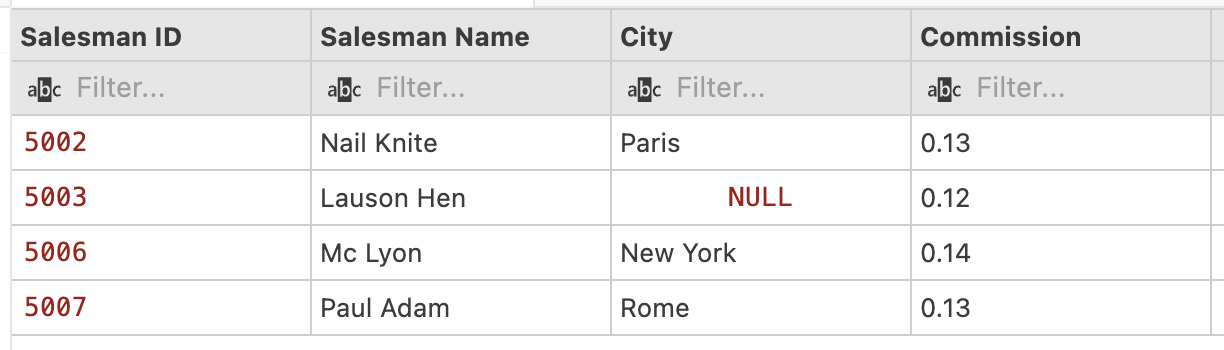
\includegraphics[width=.6\linewidth]{images/output/q3.png}
        \caption*{Salesmen with all information who gets the commission within a range of 0.12 \& 0.14}
        \label{fig:q3}
    \end{subfigure}
    \vspace*{10mm}
    \begin{subfigure}{.5\textwidth}
        \centering
        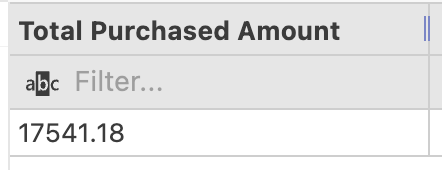
\includegraphics[width=.8\linewidth]{images/output/q4.png}
        \caption*{The total purchase amount of all orders}
        \label{fig:q4}
    \end{subfigure}
    \begin{subfigure}{.5\textwidth}
        \centering
        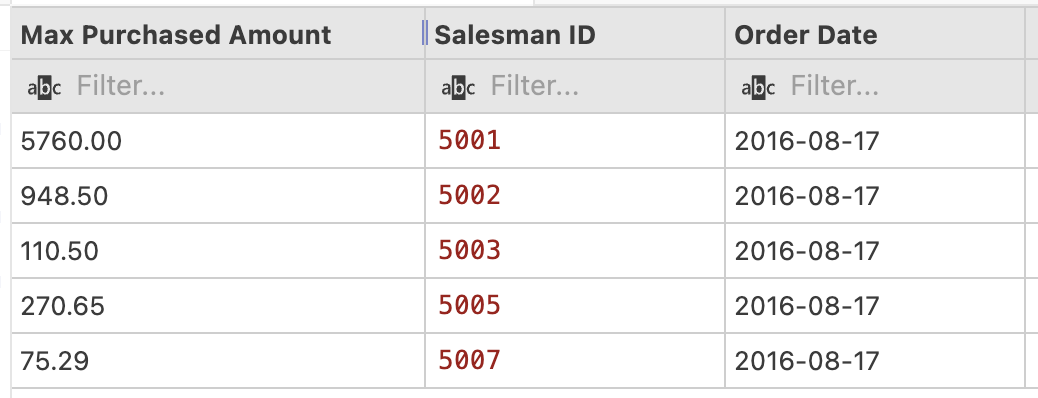
\includegraphics[width=.8\linewidth]{images/output/q5.png}
        \caption*{The highest purchase amount on date “2016-08-17” for each
            salesman with their ID}
        \label{fig:q5}
    \end{subfigure}
    \begin{subfigure}{1\textwidth}
        \centering
        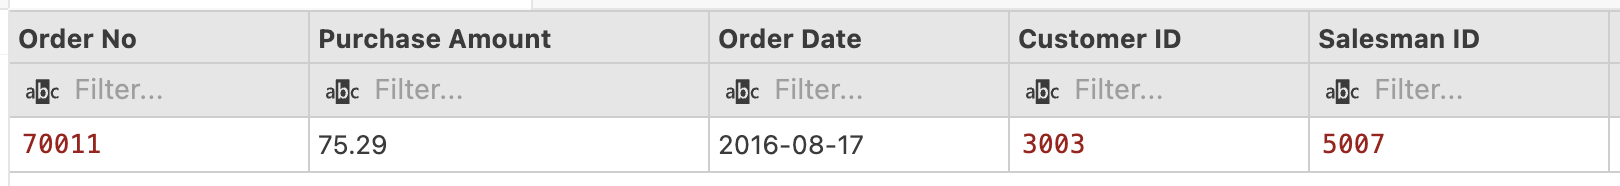
\includegraphics[width=.8\linewidth]{images/output/q6.png}
        \caption*{Display all the orders issued by the salesman “Paul Adam” from
            the orders table}
        \label{fig:q6}
    \end{subfigure}
\end{figure}
